\usetikzlibrary{arrows.meta}
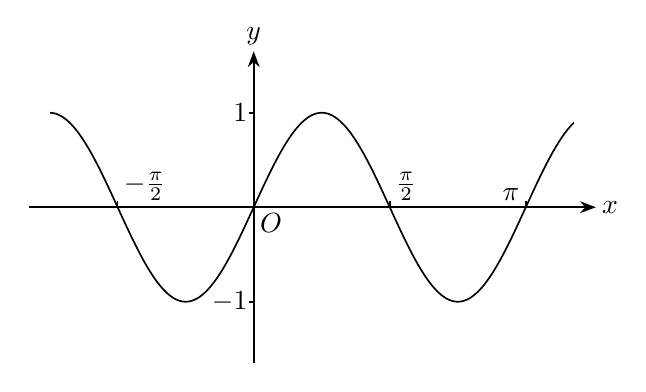
\begin{tikzpicture}[x=1.1cm,y=1.2cm,line width=.6pt,>=Stealth,font=\normalsize]
\draw[->] (-2.60,0)--(3.95,0) node[right,inner sep=0pt,xshift=2pt] {$x$};
\draw[->] (0,-1.65)--(0,1.65) node[above,inner sep=0pt,yshift=2pt] {$y$};
% x ticks: small marks
\foreach \xp in {-1.5708,1.5708,3.1416} {\draw[line width=.6pt] (\xp,0)--(\xp,0.07);}
% offset labels to avoid diagonal crossings:
% -pi/2 falling -> NE (above-right); pi/2 falling -> NE; pi rising -> NW (above-left)
\node[anchor=south west,inner sep=0pt,xshift=2pt,yshift=2pt] at (-1.5708,0) {$-\frac{\pi}{2}$};
\node[anchor=south west,inner sep=0pt,xshift=2pt,yshift=2pt] at (1.5708,0) {$\frac{\pi}{2}$};
\node[anchor=south east,inner sep=0pt,xshift=-2pt,yshift=2pt] at (3.1416,0) {$\pi$};
\node[anchor=north west,inner sep=0pt,xshift=2pt,yshift=-2pt] at (0,0) {$O$};
% y ticks
\foreach \yp in {1,-1} {\draw[line width=.6pt] (0,\yp)--(-0.06,\yp);}
\node[anchor=east,inner sep=0pt,xshift=-2pt] at (0,1) {$1$};
\node[anchor=east,inner sep=0pt,xshift=-2pt] at (0,-1) {$-1$};
% exact curve y=sin 2x
\draw[domain=-2.35:3.70,samples=260] plot (\x,{sin(2*deg(\x))});
\end{tikzpicture}
